\documentclass{beamer}
\usepackage{mathspec}
\usepackage{xeCJK}
\usepackage{graphicx}
\usepackage{hyperref}
\graphicspath{ {images/} }
\setCJKmainfont{IPAPMincho}
\setCJKsansfont{IPAGothic}
\setCJKmonofont{IPAGothic}

\setmainfont{FreeSerif}
\setsansfont{FreeSans}
\setmonofont{Latin Modern Mono}

\usetheme{DarkConsole}

\setbeamertemplate{theorems}[normal font]

\title{Máxima productividad con Tmux y Vim}
\subtitle{}
\author{Jesus Arnaiz}

\begin{document}

\begin{frame}
  \maketitle
\end{frame}

\begin{frame}{Contenido de la presentacion}
  \tableofcontents
\end{frame}

\section{Tmux}
\begin{frame}{¿Qué es Tmux?}
  \begin{enumerate}
  \item Tmux es un multiplexador de terminal
  \item Permite crear, acceder y controlar número cualquiera de terminales
  \item ... igual que GNU Screen o iTerm
  \end{enumerate}
\end{frame}

\begin{frame}{¿Por qué usar Tmux?}
  \begin{enumerate}
  \item Multiples sessiones, ventanas y paneles
  \item Persistencia de sessiones
  \item Sincronización
  \item Facil de usar y muy configurable
  \item Pair programing
  \end{enumerate}
\end{frame}
\begin{frame}
    \begin{center}
    
\includegraphics[width=\paperwidth]{whytmux}
    \end{center}
\end{frame}

\begin{frame}{¿Cómo funciona?}
  \begin{enumerate}
  \item Cliente - Servidor
  \item Sessiones
  \item Ventanas y paneles
  \end{enumerate}
\end{frame}

\begin{frame}{Demo}
  \begin{enumerate}
  \item Crear session
  \item Crear ventana
  \item split panes
  \item Sincronización de paneles
  \item Tmuxinator
  \item Pair programing
  \end{enumerate}
\end{frame}

\begin{frame}{Brico consejos}
  \begin{enumerate}
  \item Mapear tecla caps lock -> control
  \item Cambiar tmux prefix a Ctrl-a
  \item 1 Template de session por proyecto
  \item Configurar ~/.tmux.conf con vuestros propios maps y estilos
  \item Vim - Tmux navigator
  \item Explorar plugins
  \end{enumerate}
\end{frame}

\section{Vim}
\begin{frame}{Vim}
    \begin{center}
    
\includegraphics[height=\paperheight]{vimaddict}
    \end{center}
\end{frame}
\begin{frame}{¿Por qué usar Vim?}
  \begin{enumerate}
  \item Es gratis y tiene una gran comunidad detrás
  \item Muy customizable y extensible
  \item Funciona perfectamente sobre telnet y ssh
  \item Configuracion portable
  \item Muy buena documentación
  \end{enumerate}
\end{frame}

\begin{frame}{¿Cómo funciona?}
  \begin{enumerate}
  \item Modo normal, inserción y visual
  \item Movimientos
  \item Acciones
  \item Busquedas
  \item Marcas
  \item Tags
  \item Buffers
  \item Inserciones especiales
  \item Undo and Redo
  \item Registers
  \item Repeating commands
  \item split windows
  \item folding
  \end{enumerate}
\end{frame}

\begin{frame}{Plugins}
  \begin{enumerate}
  \item Vundle
  \item Solarize o Molokai
  \item NERDTree
  \item Commentary
  \item vim-surround
  \item Ctrl-P
  \item Multiple Cursors
  \item Syntastic
  \item Fugitive
  \item Tabularize
  \item easymotion
  \item Ultisnips
  \item YouCompleteMe
  \item Ack
  \item vim-tmux-navigator
  \item easyclip
  \end{enumerate}
\end{frame}

\begin{frame}{Consejos sobre vim}
  \begin{enumerate}
  \item Aprende a hablar el lenguaje vim
  \item Salir al modo normal sin usar Esc
  \item Crea tus propios maps de teclas
  \item Instala solo los plugins que vayas a usar
  \end{enumerate}
\end{frame}
\begin{frame}{Usa la ayuda}
    \begin{center}
    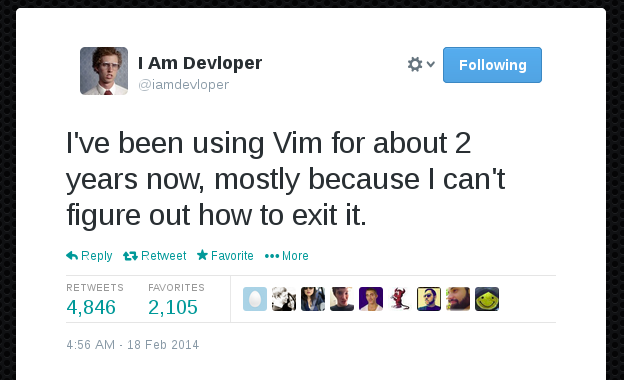
\includegraphics[width=\paperwidth]{usehelp}
    \end{center}
\end{frame}

\begin{frame}{Enlaces de interes}
  \begin{enumerate}
  \item{\href{https://github.com/j-arnaiz/codemotion-2016}{Repositorio Máxima productividad con Tmux y Vim}}
  \item{\href{http://www.vim.org/}{Vim}}
  \item{\href{https://tmux.github.io/}{Tmux}}
  \item{\href{https://github.com/tmuxinator/tmuxinator}{Tmuxinator}}
  \item{\href{http://vim.spf13.com/}{Distribución vim sfp13}}
  \end{enumerate}
\end{frame}

\begin{frame}{Ruegos y preguntas}
  \begin{enumerate}
  \item Muchas gracias por asistir
  \item Preguntas
  \end{enumerate}
\end{frame}
\end{document}
